\documentclass[paper=a4, fontsize=11pt]{scrartcl} % A4 paper and 11pt font size

%----------------------------------------------------------------------------------------
%	PACKAGES
%----------------------------------------------------------------------------------------
\usepackage[T1]{fontenc} % Use 8-bit encoding that has 256 glyphs
\usepackage{fourier} % Use the Adobe Utopia font for the document - comment this line to return to the LaTeX default
\usepackage[english]{babel} % English language/hyphenation
\usepackage{amsmath,amsfonts,amsthm} % Math packages
\usepackage{sectsty} % Allows customizing section commands
\usepackage{fancyhdr} % Custom headers and footers
\usepackage{tabularx, outlines, framed, varwidth, enumitem, graphicx, listings, color, qtree, float, subcaption, newfloat}
\usepackage[left=0.5in, right=0.5in, top=3in, bottom=.25in]{geometry}
\geometry{}

%----------------------------------------------------------------------------------------
%	SET CUSTOMIZATIONS AND FUNCTIONS
%----------------------------------------------------------------------------------------
\sectionfont{\centering \normalfont\scshape} % Make all sections centered, the default font and small caps
\pagestyle{fancyplain} % Makes all pages in the document conform to the custom headers and footers
\fancyhead{} % No page header - if you want one, create it in the same way as the footers below
\fancyfoot[L]{} % Empty left footer
\fancyfoot[C]{} % Empty center footer
\fancyfoot[R]{\thepage} % Page numbering for right footer
\renewcommand{\headrulewidth}{0pt} % Remove header underlines
\renewcommand{\footrulewidth}{0pt} % Remove footer underlines
\setlength{\headheight}{0pt} % Customize the height of the header

\DeclareFloatingEnvironment[fileext=lod]{diagram}

\numberwithin{equation}{section} % Number equations within sections (i.e. 1.1, 1.2, 2.1, 2.2 instead of 1, 2, 3, 4)
\numberwithin{figure}{section} % Number figures within sections (i.e. 1.1, 1.2, 2.1, 2.2 instead of 1, 2, 3, 4)
\numberwithin{table}{section} % Number tables within sections (i.e. 1.1, 1.2, 2.1, 2.2 instead of 1, 2, 3, 4)

\graphicspath{{./figures/}}
%\setlength\parindent{0pt} % Removes all indentation from paragraphs - comment this line for an assignment with lots of text

\makeatletter
	\newcommand*\variableheghtrulefill[1][.4\p@]
	{%
		\leavevmode
		\leaders \hrule \@height #1\relax \hfill
		\null
	}
\makeatother

\lstset
{
	language=C++,
%	basicstyle=\ttfamily,
%	keywordstyle=\color{blue}\ttfamily,
%	stringstyle=\color{red}\ttfamily,
%	commentstyle=\color{green}\ttfamily,
%	morecomment=[l][\color{magenta}]{\#}
	keywordstyle=\color{blue},
	stringstyle=\color{red},
	commentstyle=\color{green},
	morecomment=[l][\color{magenta}]{\#}
}

%----------------------------------------------------------------------------------------
%	USEFUL COMMANDS
%----------------------------------------------------------------------------------------
%	\makebox[\textwidth][c]{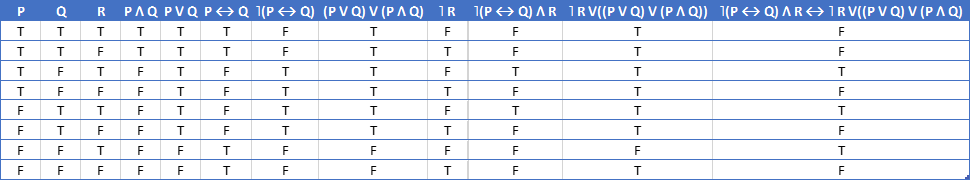
\includegraphics[width=.9\pagewidth]{p2-table}}

%	\newgeometry{top=.75in, bottom=.75in, left=.25in,right=.25in}
%	\newgeometry{top=.75in, bottom=.75in, left=1.25in,right=1.25in}

%	\lstinputlisting[firstline=4]{CMPSC360_Homework.cpp}

%\Tree
%	[.<root> [.<left> ][.<middle> ][.<right> ]]

%----------------------------------------------------------------------------------------
%	TITLE SECTION
%----------------------------------------------------------------------------------------

\newcommand{\horrule}[1]{\rule{\linewidth}{#1}} % Create horizontal rule command with 1 argument of height
% \title{Template: Homework 1}
\title{	
\normalfont \normalsize 
%\textsc{Rutgers University, Real Analysis I} \\ [25pt] % Your university, school and/or department name(s)
\horrule{0.5pt} \\[0.4cm] % Thin top horizontal rule
\huge STAT 463: Homework 4 \\ % The assignment title
\horrule{2pt} \\[0.5cm] % Thick bottom horizontal rule
}

\author{\textbf{\underline{Name:}}Kyle Salitrik | \textit{\textbf{\underline{ID\#:}} 997543474} | \textit{\textbf{\underline{PSU ID:}} kps168}} % Your name

\date{\normalsize\today} % Today's date or a custom date

\begin{document}

\maketitle % Print the title

%----------------------------------------------------------------------------------------
%	PROBLEM 1
%----------------------------------------------------------------------------------------
\newgeometry{top=.75in, bottom=.75in, left=1.25in,right=1.25in}
\section*{\variableheghtrulefill[.25ex]\quad Problem 1 \quad\variableheghtrulefill[.25ex]}
When forecasting, for $t > T \Rightarrow e_t = 0$
\begin{flalign*}
	y_{81} &= 50 - 0.7 * 3 = 47.9 &\\
	y_{82} &= 50 - 0.7 * 47.9 = 16.47 &\\
	y_{83} &= 50 - 0.7 * 16.47 = 38.471  &
\end{flalign*}

\subsection*{a)}
For $y_{81}$'s forecast see above equations.
\begin{flalign*}
	\text{PI}{y_{81}} &= X^{80}_{81} \pm 1.96*\sqrt{\hat{\sigma}^2_w * \Psi_0^2} \\
	& = 47.9 \pm 1.96 *  \sqrt{2.5^2 * 1} \\
	& = \{43, 52.8\}    &
\end{flalign*}

\subsection*{b)}
For $y_{83}$'s forecast see above equations.
\begin{flalign*}
	\text{PI}{y_{83}} &= X^{80}_{83} \pm 1.96*\sqrt{\hat{\sigma}^2_w * (\Psi_0^2 + \Psi_1^2 + \Psi_2^2)} \\
	& = 38.471 \pm 1.96 *  \sqrt{2.5^2 * (1 + 0.49 + 0.2401)} \\
	& \approx \{32.03, 44.92\}    &
\end{flalign*}

%----------------------------------------------------------------------------------------
%	PROBLEM 2
%----------------------------------------------------------------------------------------

\section*{\variableheghtrulefill[.25ex]\quad Problem 2 \quad\variableheghtrulefill[.25ex]}

\subsection*{a)}
Plotting the time series doesn't appear to show any significant trend. The plot appears to be stationary as well.

\makebox[\textwidth][c]{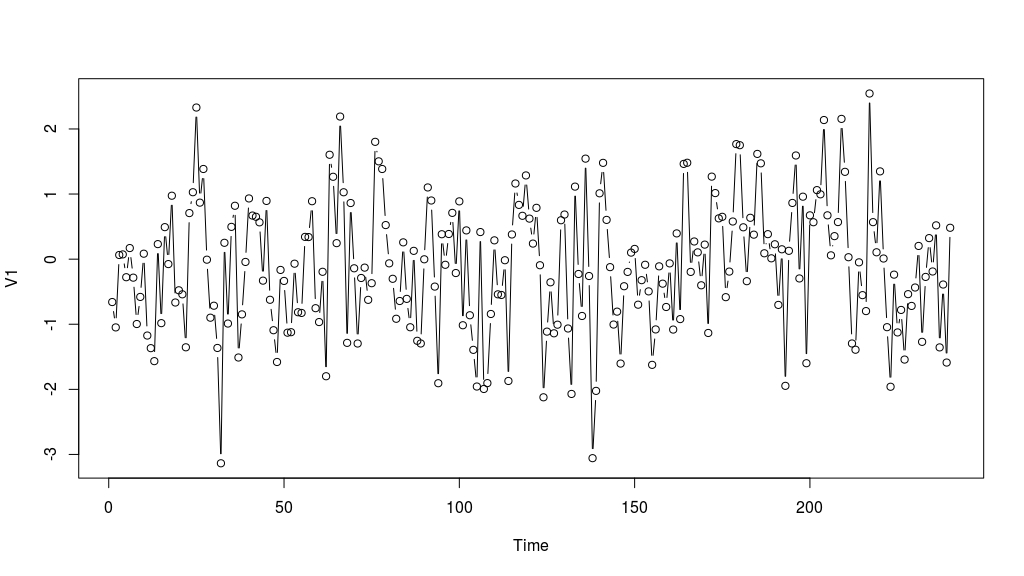
\includegraphics[scale=.5]{p2_time_series.png}}

\subsection*{b)}
Looking at the ACF and PACF plots, there is a single significant spike in each indicating that the model is possibly AR(1), MA(1) or ARMA(1,1).

\makebox[\textwidth][c]{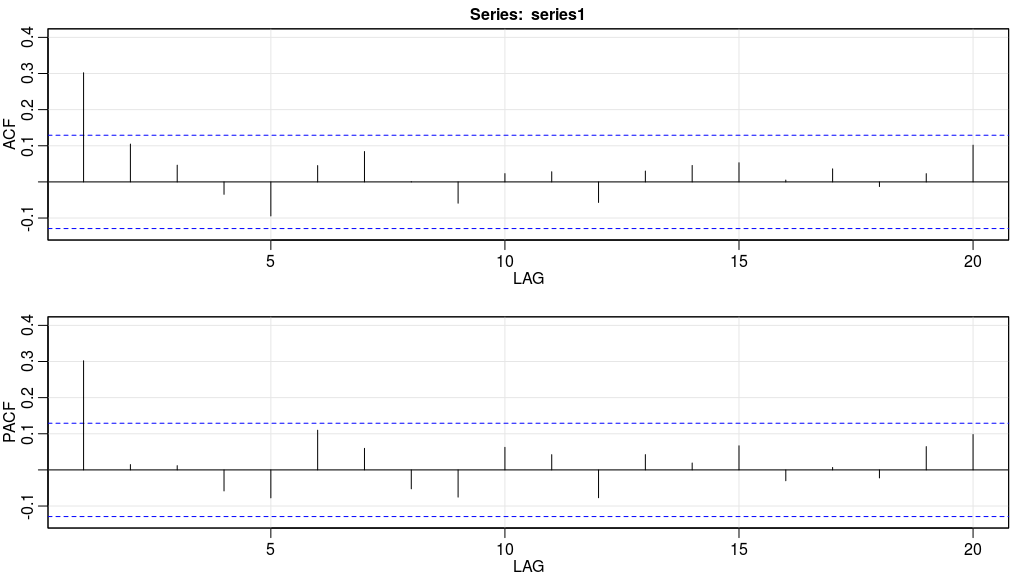
\includegraphics[scale=.5]{p2_acf_plots.png}}

\subsection*{c)}
The MA(1) model seems suitable based on the diagnostic plots. The sigma squared value is also 0.9303.

\makebox[\textwidth][c]{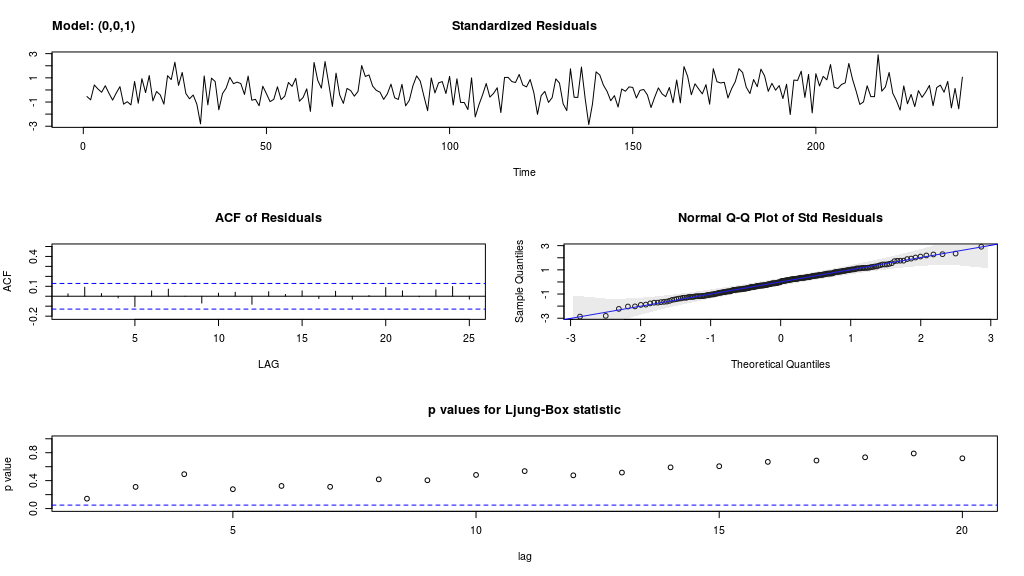
\includegraphics[scale=.5]{p2_ma1.png}}

\subsection*{d)}
While the MA(2) model may be suitable, it does have a lower sigma squared value of 0.9242.

\makebox[\textwidth][c]{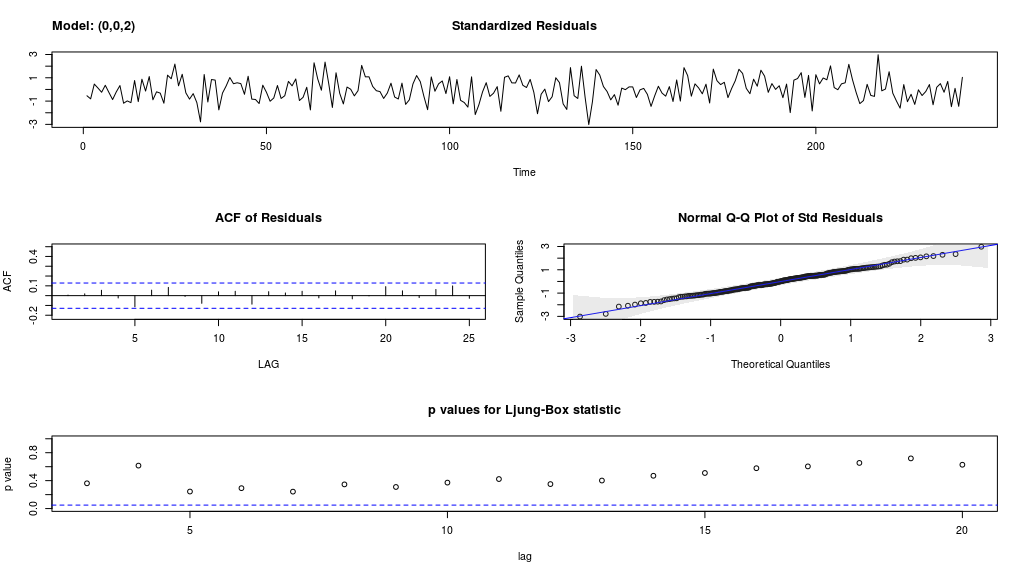
\includegraphics[scale=.5]{p2_ma2.png}}

\subsection*{e)}
In both models, the MA1 coefficient is significant, having a 0 p-value in both cases. However in the MA2 model, the p-value of the MA2 coefficient is 0.207, which is fairly insignificant, indicating that MA1 is a better option.

\subsection*{f)}
$y_t = -0.1124 + 0.2873y_{t-1} + e_t$

\subsection*{g)}
Using an ARIMA(1,0,1) model results in a sigma squared value of 0.9219, lower than the AR(1) model. However the AR(1) coefficient has a significantly lower p-value than the MA(1): 0.0877 vs 0.8212

\makebox[\textwidth][c]{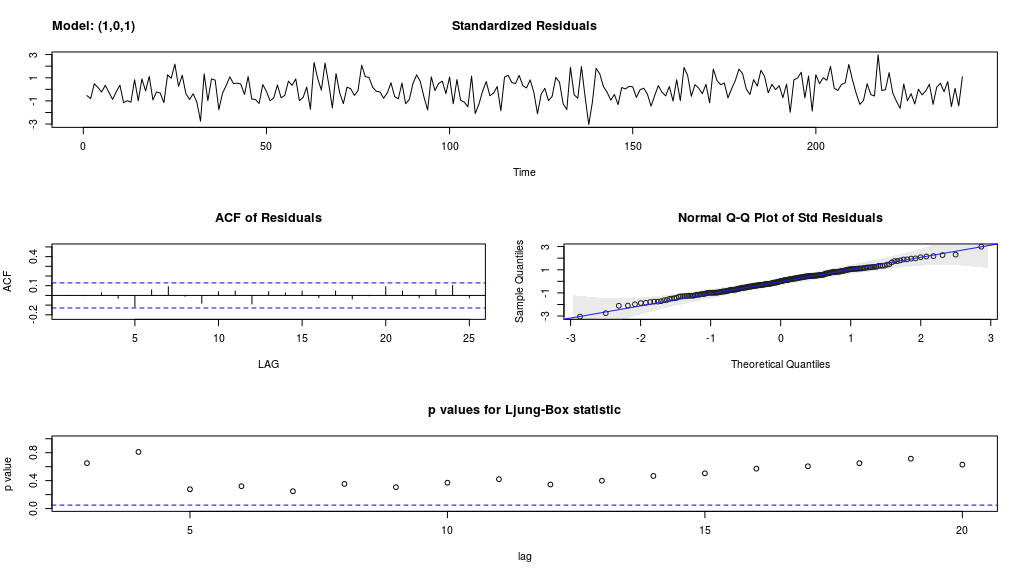
\includegraphics[scale=.5]{p2_arima11.png}}

\subsection*{h)}
Based purely on the sigma-squared values, the AR(1) model is better. In this model the coefficient is also more significant than either coefficient in the ARIMA(1,0,1) model.
\subsection*{i)}
\lstinputlisting[language=]{listings/p2_sarima_output.txt}

\subsection*{j)}
The values converge due to the properties of the time series model itself. At infinite time, the values of the prediction of the time series will converge to the mean of the series.

%----------------------------------------------------------------------------------------
%	PROBLEM 3
%----------------------------------------------------------------------------------------

\section*{\variableheghtrulefill[.25ex]\quad Problem 3 \quad\variableheghtrulefill[.25ex]}
\subsection*{a)}
Looking at the time series, there appears to be a seasonality to the data.

\makebox[\textwidth][c]{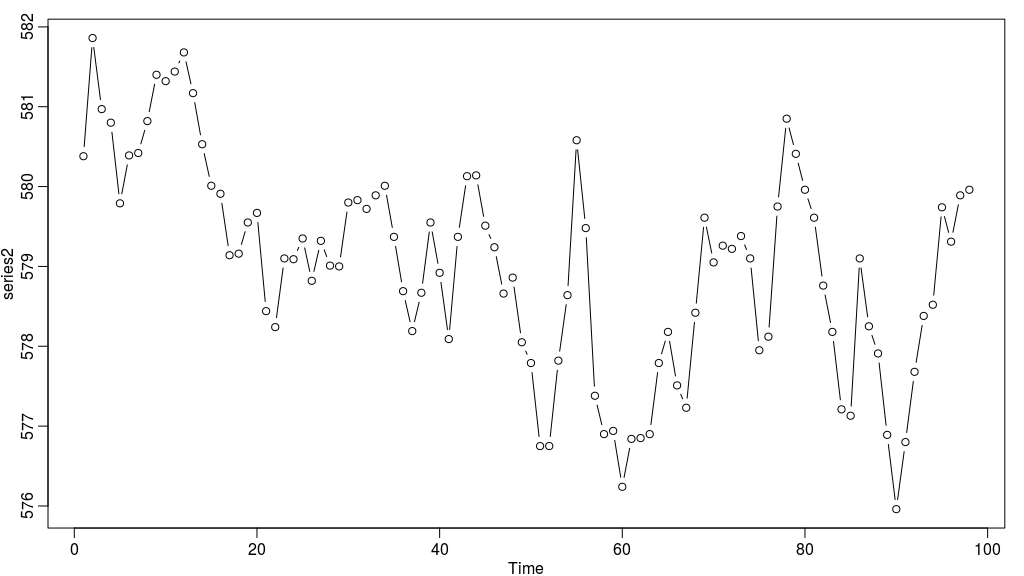
\includegraphics[scale=.5]{p3_time_series.png}}

\subsection*{b)}
Looking at the ACF and PACF plots, there is a single significant spike in each indicating that the model is possibly AR(2) or anywhere from MA(1) to MA(9).

\makebox[\textwidth][c]{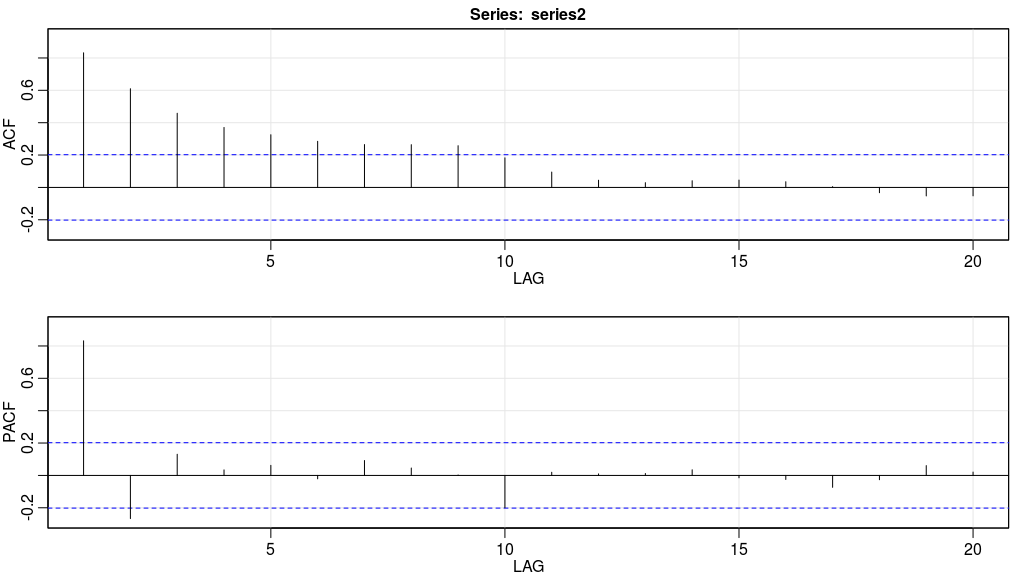
\includegraphics[scale=.5]{p3_acf_plots.png}}

\subsection*{c)}
The AR(2) model appears to be fairly suitable for use as all of the points within the Ljung-Box plot and the ACF of residuals are insignificant.

\makebox[\textwidth][c]{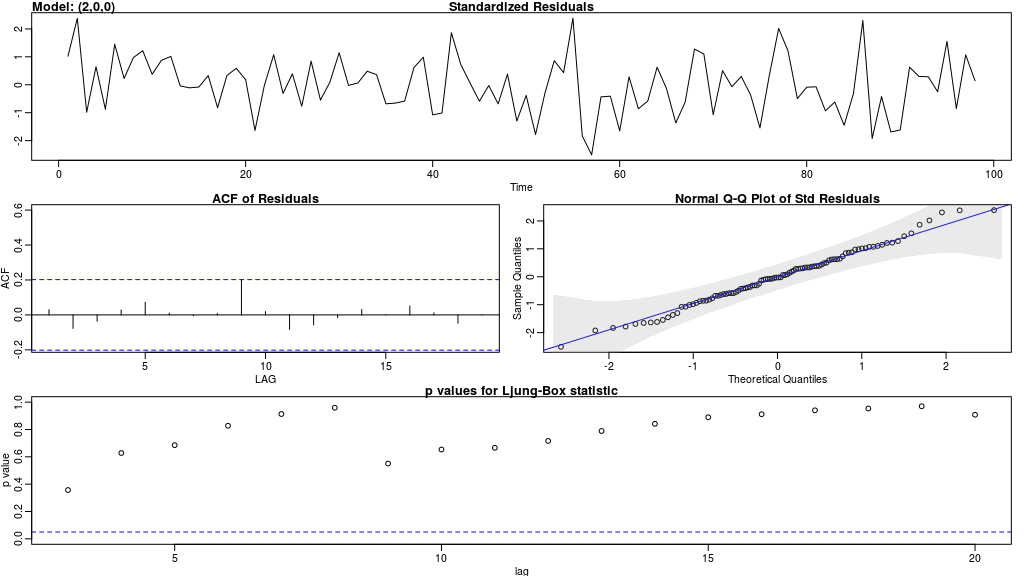
\includegraphics[scale=.5]{p3_ar2.png}}

\subsection*{d)}
Based on the results of the sarima function, the AR(1) coefficient has a p-value of 0 and the AR(2) coefficient has a p-value of 0.0151. Depending on the threshold one wants to use, these both may be significant or only the AR(1).

\subsection*{e)}
Using the given equation, we can estimate the intercept to be:
$\delta = 579.0473(1 - 1.0436 + 0.2495) \approx 119.23$

And the regression equation is as follows:
$y_t = 119.23 + 1.0436*y_{t-1} - 0.2495*y_{t-2} + e_t$ 

\subsection*{f)}
For the estimates:

\begin{flalign*}
	y_{99} &= 119.23 + 1.0436 * 579.89 - 0.2495 * 579.96 = 579.70 &\\
	y_{100} &= 119.23 + 1.0436 * 579.70 - 0.2495 * 579.96 = 579.50 &\\
	y_{101} &= 119.23 + 1.0436 * 579.50  - 0.2495 * 579.70 = 579.36 &
\end{flalign*}



%----------------------------------------------------------------------------------------
%	PROBLEM 4
%----------------------------------------------------------------------------------------

\section*{\variableheghtrulefill[.25ex]\quad Problem 4 \quad\variableheghtrulefill[.25ex]}

\subsection*{a)}
There appears to be a yearly trend for the price of flour, however it seems that each year is mostly independent.

\makebox[\textwidth][c]{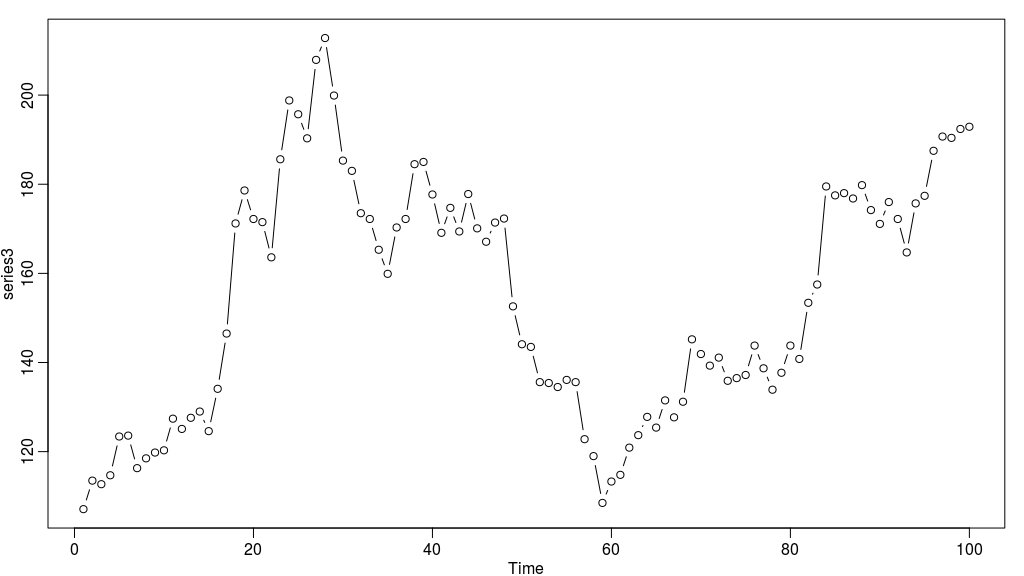
\includegraphics[scale=.5]{p4_time_series.png}}

\subsection*{b)}
An AR(1) model may apply based on the PACF, however it's more likely that a high order MA model may fit best.

\makebox[\textwidth][c]{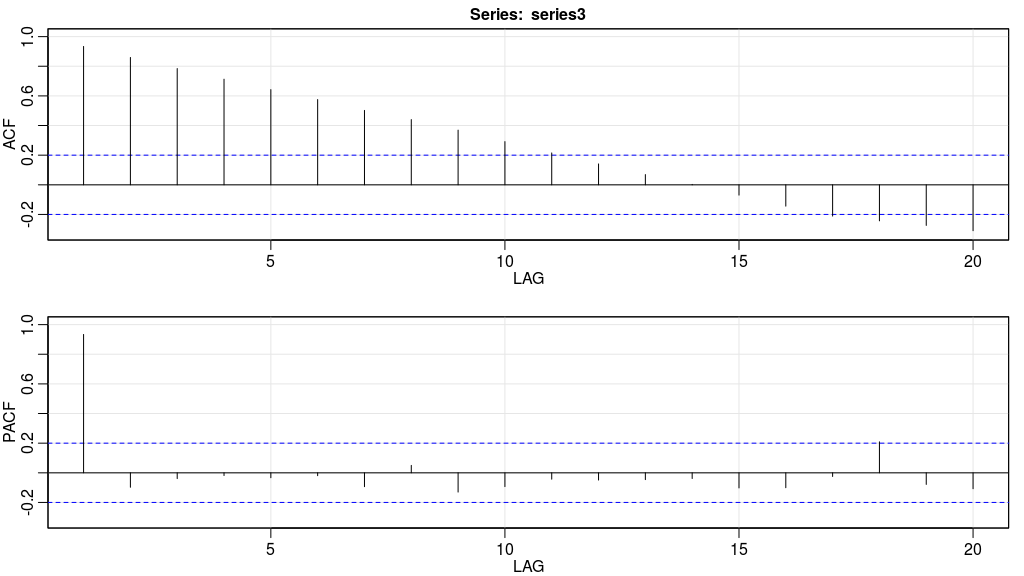
\includegraphics[scale=.5]{p4_acf_plots.png}}

\subsection*{c)}
For the difference, there is no significant spikes, meaning that no time series related models may fit the first difference of the data.

\makebox[\textwidth][c]{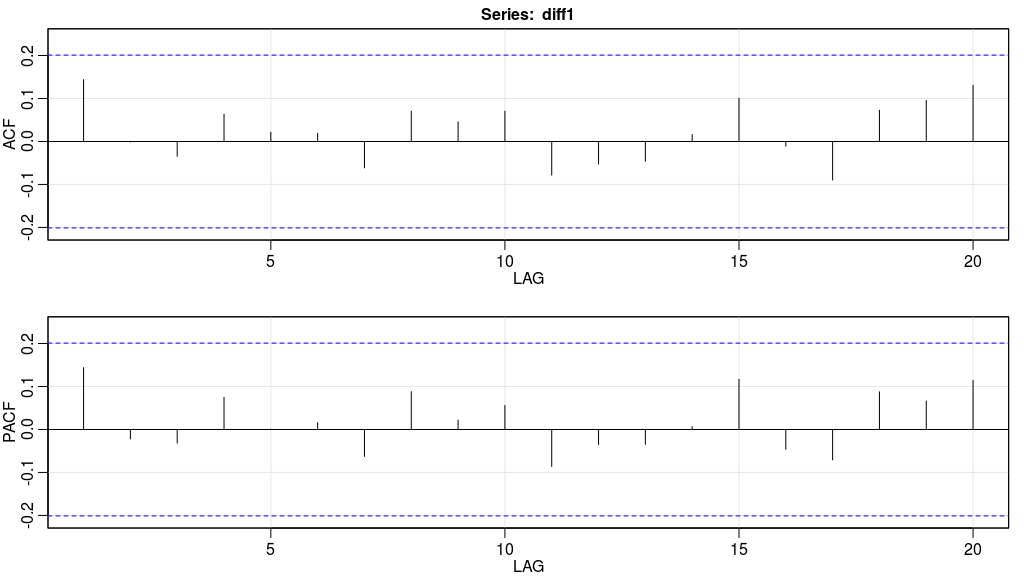
\includegraphics[scale=.5]{p4_diff_plot.png}}




\end{document}